\documentclass[12pt]{article}
\usepackage{amsthm,amssymb,amsmath,amsfonts}
\usepackage[a4paper, top=25mm, bottom=30mm, left=25mm, right=25mm]{geometry}
\usepackage[pagebackref=false,colorlinks,linkcolor=black,citecolor=black]{hyperref}
\usepackage[nameinlink]{cleveref}
 \AtBeginDocument{%
    \crefname{equation}{برابری}{equations}%
    \crefname{chapter}{فصل}{chapters}%
    \crefname{section}{بخش}{sections}%
    \crefname{appendix}{پیوست}{appendices}%
    \crefname{enumi}{مورد}{items}%
    \crefname{footnote}{زیرنویس}{footnotes}%
    \crefname{figure}{شکل}{figures}%
    \crefname{table}{جدول}{tables}%
    \crefname{theorem}{قضیه}{theorems}%
    \crefname{lemma}{لم}{lemmas}%
    \crefname{corollary}{نتیجه}{corollaries}%
    \crefname{proposition}{گزاره}{propositions}%
    \crefname{definition}{تعریف}{definitions}%
    \crefname{result}{نتیجه}{results}%
    \crefname{example}{مثال}{examples}%
    \crefname{remark}{نکته}{remarks}%
    \crefname{note}{یادداشت}{notes}%
    \crefname{observation}{مشاهده}{observations}%
    \crefname{algorithm}{الگوریتم}{algorithms}%
    \crefname{cproof}{برهان}{cproofs}%
}

\usepackage{tikz}
\usepackage{graphicx}
\usepackage{booktabs}
\usepackage{color}
\usepackage{graphicx}
\usepackage{subcaption}

\usepackage{setspace}
\doublespacing

\usepackage{titletoc}
\usepackage{tocloft}
\usepackage{enumitem}
\usepackage{amsmath, amssymb}
\usepackage{algorithm}
\usepackage[noend]{algorithmic}
\renewcommand{\algorithmicrequire}{\textbf{Input:}}
\renewcommand{\algorithmicensure}{\textbf{Output:}}

\usepackage{tabularx}
\makeatletter
\newcommand{\multiline}[1]{%
  \begin{tabularx}{\dimexpr\linewidth-\ALG@thistlm}[t]{@{}X@{}}
    #1
  \end{tabularx}
}
\makeatother

\usepackage{float}
\usepackage{verbatim}
\makeindex
\usepackage{sectsty}
\usepackage{xepersian}
\SepMark{-}
\settextfont[Scale=1.2,Path=fonts/,BoldFont=B Nazanin Bold.ttf]{B Nazanin.ttf}
\setlatintextfont{Times New Roman}
\renewcommand{\labelitemi}{$\bullet$}

\theoremstyle{definition}
\newtheorem{definition}{تعریف}[section]
\newtheorem{remark}[definition]{نکته}
\newtheorem{note}[definition]{یادداشت}
\newtheorem{example}[definition]{نمونه}
\newtheorem{question}[definition]{سوال}
\newtheorem{remember}[definition]{یاداوری}
\newtheorem{observation}[definition]{مشاهده}
\theoremstyle{theorem}
\newtheorem{theorem}[definition]{قضیه}
\newtheorem{lemma}[definition]{لم}
\newtheorem{proposition}[definition]{گزاره}
\newtheorem{corollary}[definition]{نتیجه}
\newtheorem*{cproof}{برهان}




\begin{document}
\fontsize{12pt}{14pt}\selectfont

\begin{minipage}{0.1\textwidth}

\includegraphics[width=3cm]{etc/IUST}
\end{minipage}%
\hfill%
\begin{minipage}{0.6\textwidth}\centering
\fontsize{13pt}{13pt}\selectfont
به‌ نام خدا \\
\textbf{درس یادگیری عمیق} \\
\textbf{تمرین سری ششم}\\
استاد درس : دکتر محمدرضا محمدی \\
دستیاران :  مهدی خورشا، سید محمد موسوی،\\ امیرحسین نمازی
\\
\vspace{0.25cm}
\begingroup
\fontsize{11pt}{11pt}\selectfont
دانشگاه علم و صنعت ایران، دانشکده مهندسی کامپیوتر \\
نیمسال دوم تحصیلی 1403 - 1404 \\
\endgroup
\end{minipage}%
\hfill%
\begin{minipage}{0.1\textwidth}

\end{minipage}

\vspace{0.5cm}

\noindent\rule{\textwidth}{1pt}

\centering {\fontsize{18}{22}\selectfont \textbf{مهلت تحویل : 1403/12/22 }}\\
{\fontsize{14}{22}\selectfont \textbf{لطفا به نکات موجود در سند قوانین انجام و تحویل تمرین ها دقت فرمایید. }}

\begin{enumerate}

    \section*{سوالات تئوری}
    \item 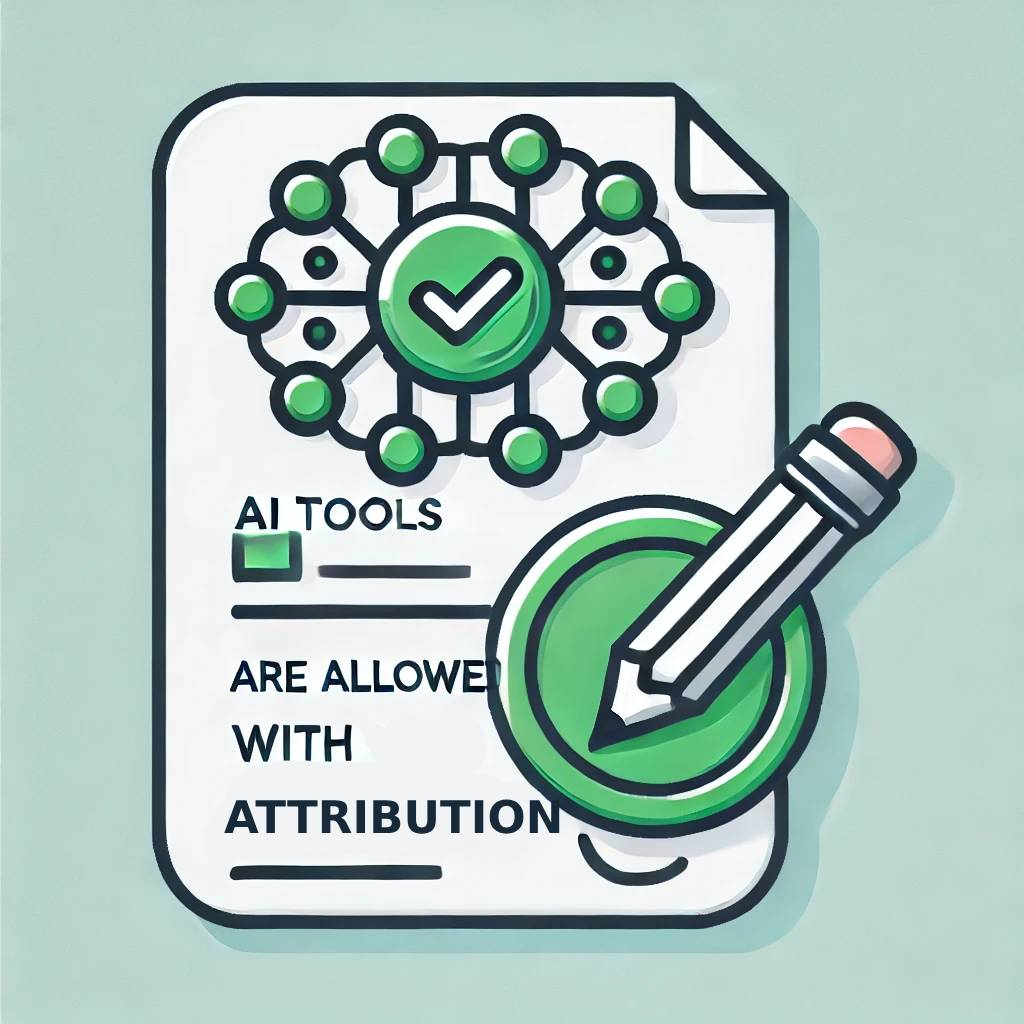
\includegraphics[width=1cm]{figs/Allowed_with_contributino.jpg}
     فرض کنید $f: \mathbb{R}^n \to \mathbb{R}$ یک تابع مشتق‌پذیر پیوسته به فرم زیر است:

    \[
    f(x) = \exp(-\|Ax - b\|^2) + \sin\left(\sum_{i=1}^{n} c_i x_i^2\right)
    \]
    
    که:
    \begin{itemize}
        \item $A \in \mathbb{R}^{n \times n}$ یک ماتریس با مرتبه کامل است.
        \item $b \in \mathbb{R}^n$ یک بردار بایاس است.
        \item $c_i \in \mathbb{R}$ ضرایب ثابت نامنفی یا صفر هستند.
    \end{itemize}
    
    ثابت کنید که برای هر مقدار $\epsilon > 0$ حداقل یک شبکه پرسپترون چند لایه $F(x)$ با تعداد محدودی نورون وجود دارد که بتواند تابع $f(x)$ را به‌طور دلخواه در یک دامنه فشرده $D \subset \mathbb{R}^n$ تقریب بزند به‌طوری‌که:(15 نمره)
    
    \[
    \| f(x) - F(x) \|_{L_2} < \epsilon
    \]
    
    \textbf{راهنما:} برای حل این مسئله ابتدا تابع $f(x)$ را به دو بخش نمایی و سینوسی تقسیم کنید. سپس با استفاده از مبانی تئوری و شبکه‌های عصبی چندلایه، هر بخش را به‌طور جداگانه تقریب بزنید. می‌توانید از منابع زیر برای اثبات خود کمک بگیرید:

    \lr{
    \begin{itemize}
        \item \href{https://cognitivemedium.com/magic_paper/assets/Hornik.pdf}{\lr{Multilayer Feedforward Networks are Universal Approximators}}
        \item \href{https://hal.science/hal-03753170/file/Cybenko1989.pdf}{\lr{Approximation by superpositions of a sigmoidal function}}
    \end{itemize}
    }

    \textcolor{blue}{
    \lr{
        $$
            \begin{gathered}
            K \subset \mathbb{R}^d(d \geq 1), K \text { compact, } \\
            \sigma: \mathbb{R} \rightarrow \mathbb{R}, \lim _{t \rightarrow-\infty} \sigma(t)=0, \lim _{t \rightarrow+\infty} \sigma(t)=1 . \\
            \mathcal{G}=\left\{G(x)=\sum_{j=1}^r \alpha_j \sigma\left(w_j \cdot x+\theta_j\right): r \in \mathbb{N}, \alpha_j, \theta_j \in \mathbb{R}, w_j \in \mathbb{R}^d\right\} . \\
            \overline{\mathcal{G}}^{\|\cdot\|_{\infty}=C(K) .} \\
            \exists \Lambda \in C(K)^* \backslash\{0\}, \Lambda(G)=\{0\} \Rightarrow \\
            \exists \mu \neq 0(\text { finite signed }): \Lambda(g)=\int_K g d \mu, \\
            \int_K \sigma(w \cdot x+\theta) d \mu(x)=0 \forall w, \theta . \\
            \sigma_k(t)=\sigma(k t), \sigma_k \rightarrow 1[0, \infty) ; \int_K 1(w \cdot x+\theta \geq 0\} d \mu=0, \\
            \mu\left(H_{w, \theta} \cap K\right)=0 \forall w, \theta\left(H_{w, \theta}=\{x: w x+\theta \geq 0\}\right) . \\
            \Rightarrow \mu=0\left(\text { half-spaces generate } \mathcal{B}\left(\mathbb{R}^d\right)\right) \perp \\
            \Rightarrow \Lambda=0, \bar{G}=C(K) . \\
            \forall f \in C(K), \forall \varepsilon>0, \exists r, \alpha_j, w_j, \theta_j: \\
            \sup \left|f(x)-\sum_{j=1}^r \alpha_j \sigma\left(w_j x+\theta_j\right)\right|<\varepsilon . \\
            x \in K \\
            f: K \rightarrow \mathbb{R}^m, f=\left(f_1, \ldots, f_m\right), \varepsilon>0: \\
            \exists F_k \in \mathcal{G}, \sup _x\left|f_k(x)-F_k(x)\right|<\varepsilon / \sqrt{m}, \\
            F=\left(F_1, \ldots, F_m\right), \sup _{x \in K}\|f(x)-F(x)\|_2<\varepsilon
            \end{gathered}
        $$}}
    \textcolor{blue}{
        در این برهان، نخست مجموعه تمام توابع شبکه عصبی تک لایه با فعال‌ساز سیگموید را تعریف می‌کنیم؛ هر تابع این مجموعه ترکیبی خطی محدودی از سیگمویدهای $\sigma(w.x+\theta)$ است. گام بعدی نشان می‌دهد که اگر تابع خطی پیوسته‌ای روی فضای توابع پیوسته $C(K)$ وجود داشته باشد که بر تمام اعضای این مجموعه صفر شود، آن تابع باید انتگرال نسبت به یک اندازه $Signed \mu$ باشد که شرط $∫\sigma(w.x+\theta)d\mu=0$ را برای همه $(w,\theta)$ برآورده می‌کند. با بزرگ‌کردن شیب سیگموید، $\sigma(kt)$ به تابع پله واحد همگرا شده و نتیجه می‌دهد اندازه $H_(w,\theta)$ روی هر نیم‌فضای $H_(w,\theta)$ صفر است. چون نیم‌فضاها $\sigma$ جبر بورل را تولید می‌کنند، تنها اندازه ممکن $\mu$ صفر است؛ از این تناقض می‌فهمیم هیچ تابع خطی غیرصفر نمی‌تواند کل مجموعه شبکه‌ها را نقض کند. طبق قضیه هان باناک، این امر به چگالی مجموعه شبکه‌ها در $C(K)$ منتهی می‌شود؛ بنابراین برای هر تابع پیوسته و هر $\epsilon>0$، شبکه‌ای با تعداد متناهی نورون وجود دارد که خطای یکنواخت آن از $\epsilon$کمتر است. در پایان، برای خروجی‌های برداری $R^m$، هر مؤلفه جداگانه تقریب می‌شود و با کنار هم گذاشتن لایه‌های پنهان، شبکه‌ای با خطای $\epsilon$ در نرم اقلیدسی بر کل دامنه فشرده حاصل می‌شود.}    
    
    \item 
\includegraphics[width=1cm]{figs/Forbidden_AI.jpg}
   اثبات کنید که افزودن یک ترم \( L_2 \) به تابع هزینه:
    \[
    R_\lambda (F) = R(F) + \lambda \| W \|_2^2
    \]
    واریانس مدل را کاهش داده و به بهبود تعمیم‌دهی کمک می‌کند. تأثیر پارامتر \( \lambda \) بر کران تعمیم (\lr{generalization bound}) را استخراج کنید(10 نمره).
    
    \textcolor{blue}{
    $$
        \begin{gathered}
        \hat{R}_n(F)=\frac{1}{n} \sum_{i=1}^n \ell\left(F\left(x_i\right), y_i\right), \quad \mathcal{R}_\lambda(F)=\hat{R}_n(F)+\lambda\|W\|_2^2, \\
        F^*=\underset{F \in \mathcal{H}}{\arg \min \mathcal{R}_\lambda(F), \quad \ell \in[0,1],} \\
        \lambda\left\|W^*\right\|_2^2 \leq 1 \Rightarrow\left\|W^*\right\|_2 \leq \frac{1}{\sqrt{\lambda}}, \\
        \widehat{\Re}_n\left(\mathcal{H}_B\right) \leq \frac{L_\sigma R B}{\sqrt{n}}\left(B=\frac{1}{\sqrt{\lambda}}\right) \Rightarrow \widehat{\Re}_n\left(\mathcal{H}_B\right) \leq \frac{L_\sigma R}{\sqrt{n \lambda}}, \\
        \operatorname{Pr}\left(R\left(F^*\right) \leq \hat{R}_n\left(F^*\right)+\frac{2 L_\sigma R}{\sqrt{n \lambda}}+3 \sqrt{\left.\frac{\log (2 / \delta)}{2 n}\right)} \geq 1-\delta,\right. \\
        R\left(F^*\right) \leq \hat{R}_n\left(F^*\right)+\frac{2 L_\sigma R}{\sqrt{n \lambda}}+3 \sqrt{\frac{\log (2 / \delta)}{2 n}} .
        \end{gathered}
    $$
    }
    \textcolor{blue}{
    در این اثبات، ابتدا ریسک تجربی منظم‌شده را تعریف می‌کنیم. این ریسک شامل دو بخش است: میانگین خطاهای مدل روی داده‌های آموزش و یک جمله‌ی جریمه که به‌صورت $\lambda\|W\|_2^2$ تعریف می‌شود. این جمله باعث می‌شود که مدل‌هایی با وزن‌های بزرگ‌تر کمتر ترجیح داده شوند و در نتیجه پیچیدگی مدل کاهش یابد.
    سپس نشان داده می‌شود که اگر این تابع هزینه را کمینه کنیم، نورم وزن‌های به‌دست‌آمده حداکثر برابر با $1/√\lambda$ خواهد بود. به‌عبارت‌دیگر، بزرگ‌تر شدن $\lambda$ باعث می‌شود مدل ساده‌تری انتخاب شود.
    در ادامه، با استفاده از ویژگی‌هایی مثل محدود بودن داده‌ها و پیوستگی تابع فعال‌سازی (مثلاً سیگموید)، می‌توان پیچیدگی مدل را به کمک پیچیدگی «رادماخر» اندازه‌گیری کرد. نتیجه این است که هرچه $\lambda$ بیشتر باشد، این پیچیدگی کمتر می‌شود.
    در نهایت، با استفاده از نابرابری‌های آماری (مثل نابرابری بوسکه)، کرانی برای ریسک واقعی مدل به دست می‌آید که شامل سه جمله است: ریسک تجربی، یک جمله‌ی مربوط به پیچیدگی مدل (که به $\lambda$ وابسته است)، و یک جمله‌ی تصادفی مربوط به تعداد داده‌ها و سطح اطمینان. این کران نشان می‌دهد که اضافه کردن جمله‌ی منظم‌ساز باعث کاهش واریانس مدل و بهبود تعمیم آن روی داده‌های جدید می‌شود، هرچند ممکن است کمی دقت مدل روی داده‌های آموزش را کاهش دهد. بنابراین باید $\lambda$ را با دقت و بر اساس داده‌های اعتبارسنجی تنظیم کرد تا بین بایاس و واریانس تعادل برقرار شود.}


    \item 
\includegraphics[width=1cm]{figs/Forbidden_AI.jpg}
    تصور کنید چند سال از فارغ‌التحصیلی شما گذشته و حالا در یک شرکت مشغول به کار هستید. به این نتیجه رسیده‌اید که به‌جای صعود در مسیر شغلی دیگران، کسب‌وکار شخصی خود را راه‌اندازی کنید. شما یک وب‌سایت آموزشی مفید و الهام‌بخش ساخته‌اید که حالا بازدیدکنندگان زیادی دارد و می‌خواهید از طریق تبلیغات آنلاین درآمد کسب کنید(15 نمره).

    برای کسب حداکثر درآمد از تبلیغات، به‌جای نمایش تصادفی تبلیغات، از یک سیستم حراجی استفاده می‌کنید که بهترین تبلیغات را برای هر موقعیت انتخاب می‌کند. اطلاعات تبلیغات در جدولی ثبت می‌شود که شامل موارد زیر است:
    
    \begin{itemize}
        \item \textbf{\lr{adv\_id}:} شناسه تبلیغ‌دهنده
        \item \textbf{\lr{cam\_id}:} شناسه کمپین تبلیغاتی
        \item \textbf{\lr{bid}:} مبلغ پیشنهادی برای هر کلیک یا اقدام
        \item \textbf{\lr{type}:} نوع درآمد (کلیک یا اقدام خاص)
        \item \textbf{\lr{pos\_id}:} موقعیت تبلیغ در سایت
        \item \textbf{\lr{ad\_id}:} شناسه تبلیغ
        \item \textbf{\lr{views}:} تعداد نمایش تبلیغ
        \item \textbf{\lr{clicks}:} تعداد کلیک‌ها روی تبلیغ
        \item \textbf{\lr{actions}:} تعداد اقدامات انجام‌شده پس از کلیک
        \item \textbf{\lr{week\_id}:} زمان جمع‌آوری داده‌ها (بر اساس هفته)
    \end{itemize}
    
    \begin{table}[h!]
        \centering
        \begin{tabular}{|c|c|c|c|c|c|c|c|c|c|}
            \hline
            \textbf{\lr{adv id}} & \textbf{\lr{cam id}} & \textbf{\lr{bid}} & \textbf{\lr{type}} & \textbf{\lr{pos id}} & \textbf{\lr{ad id}} & \textbf{\lr{views}} & \textbf{\lr{clicks}} & \textbf{\lr{actions}} & \textbf{\lr{week id}} \\
            \hline
            1234 & 6575 & 1000 & \lr{Click}  & 10 & 8975 & 15436 & 15 & 0 & 1735115563 \\
            1234 & 6575 & 1000 & \lr{Click}  & 13 & 6735 & 18466 & 10 & 0 & 1735115563 \\
            4321 & 9876 & 9000 & \lr{Action} & 78 & 7185 & 10321 & 20 & 2 & 1735124569 \\
            5678 & 4532 &  500 & \lr{Click}  &  5 & 1024 & 21000 & 25 & 0 & 1735114563 \\
            2345 & 3456 & 2000 & \lr{Click}  & 20 & 2341 & 18000 & 30 & 0 & 1735118563 \\
            7890 & 7654 & 8000 & \lr{Action} & 25 & 6523 & 12000 & 18 & 5 & 1735134563 \\
            \hline
        \end{tabular}
    \end{table}
    ﺑﺎ ﺍﺳﺘﻔﺎﺩﻩ ﺍﺯ ﺍﯾﻦ ﺩﺍده ﻫﺎ ﻭ ﻓﺮﻣﻮﻝﻫﺎﯼ ﺑﻬﯿنه ﺳﺎﺯﯼ ﮐﻪ ﺩﺭ ﺍﺩﺍﻣﻪ ﺍﺭﺍﺋﻪ ﺷﺪﻩ ﺍﺳﺖ، می‌توانید ﺍﻧﺘﺨﺎﺏ ﺗﺒﻠﯿﻐﺎﺕ ﺭﺍ ﺩﺭ ﺟﺎیگاه ﻫﺎﯼ ﻣﺨﺘﻠﻒ ﺑﻬﯿﻨﻪ ﮐﻨﯿﺪ ﺗﺎ ﺩﺭﺁﻣﺪ ﺷﻤﺎ ﺣﺪﺍﮐﺜﺮ ﺷﻮﺩ. ﺑﻪ ﺍﯾﻦ ﺭﻭﺍﺑﻂ ﺩﻗﺖ ﮐﻨﯿﺪ ﻭ سعیﮐﻨﯿﺪ ﺩﺭﮎ ﮐﻨﯿﺪ که ﭼﺮﺍ ﺍﯾﻦ ﻓﺮﻣﻮﻝ ﻫﺎ می ﺗﻮﺍﻧﻨﺪ ﺑﻪ ﺍﻧﺘﺨﺎﺏ ﺗﺒﻠﯿﻐﺎﺗ ﺑﺎ ﺑﯿﺸﺘﺮﯾﻦ ﺩﺭﺁﻣﺪ ﻣﻮﺭﺩ ﺍﻧﺘﻈﺎﺭﮐمک ﮐﻨﻨﺪ.
    
    \textbf{فرمول بهینه‌سازی تبلیغات کلیکی}
    \[
    \text{\lr{For each position}} (p), \text{ :\lr{select}} \arg\max_{ad \in A(p)} (bid_{ad} \times ctr(ad, p))
    \]
    
    \textbf{فرمول بهینه‌سازی تبلیغات اکشنی}
    \[
    \text{\lr{For each position}} (p), \text{ :$select$ } \arg\max_{ad \in A(p)} (bid_{ad} \times ctr(ad, p) \times cvr_{ad})
    \]
    
    \begin{itemize}
        \item \( A(p) \): مجموعه تبلیغاتی که امکان نمایش در جایگاه \( p \) دارند.
        \item \( bid_{ad} \): مبلغی که تبلیغ‌دهنده برای هر کلیک پرداخت می‌کند.
        \item \( ctr(ad, p) \): احتمال کلیک کاربر بر روی تبلیغ \( ad \) در جایگاه \( p \) (نرخ کلیک).
        \item \( cvr_{ad} \): احتمال انجام اکشن توسط کاربر پس از کلیک روی تبلیغ.
    \end{itemize}
    
    فرض کنید مدل‌های آموزش داده شده در مواجهه با ورودی‌های ناشناخته (مانند تبلیغات، کمپین‌ها یا تبلیغ‌دهندگان جدید)، به‌صورت میانگین‌گیری سیستمایتک عمل می‌کنند. به طور مشخص، اگر یک تبلیغ جدید باشد اما کمپین مرتبط با آن قبلاً در سیستم دیده شده باشد، \( CTR \) و \( CVR \) آن تبلیغ به‌صورت میانگین وزنی از مقادیر مربوط به تبلیغات قبلی آن کمپین محاسبه می‌شود.
    
    \textbf{الف)}
    یکی از مهم‌ترین مراحل در فرآیند آموزش هر مدل یادگیری ماشین، تقسیم‌بندی داده‌ها به مجموعه‌های \lr{Train}، \lr{Dev}، \lr{Train-Dev} و \lr{Test} است. این کار به ما کمک می‌کند تا عملکرد مدل را بر روی توزیع داده‌های مختلف بررسی کنیم. در این مسئله خاص چطور این‌کار را باید انجام داد و در انتخاب این مجموعه‌ها به چه نکاتی باید توجه داشت؟

    \textcolor{blue}{
    الف) چگونه داده ها را به مجموعه های \lr{Train}، \lr{Test} و \lr{Dev} تقسیم کنیم.\\
    \begin{enumerate}
        \item تقسیم تصادفی در مقابل تقسیم زمانی(\lr{Time-Based Split}):\\
            \begin{itemize}
                \item اگر رفتار کاربران، تبلیغ کنندگان یا مبلغ هاي پیشنهادي (\lr{bids}) در طول زمان به شکل قابل ملاحظه اي تغییر
                کند (اتفاقی که در دنیاي واقعی تبلیغات بسیار معمول است)، استفاده از یک تقسیم مبتنی بر زمان رویکرد
                 واقعی تري خواهد بود.
                 \begin{itemize}
                     \item مثال :استفاده از داده هاي ماه ژانویه تا مارس براي آموزش(\lr{Train}) ، آوریل براي توسعه (\lr{Dev})
                        و مه براي آزمون.(\lr{Test})
                 \end{itemize}
                 \item اگرالگوهاي زمانی قوي درداده هاوجودنداشته باشدیانگرانی ازنشت داده درطول زمان نداشته باشیم،
                تقسیم تصادفی میتواند کفایت کند. بااینحال، تقسیم تصادفی ممکن است تغییرات زمانی متداول در
                 تبلیغات را پنهان کند.
            \end{itemize}
        \item حفظ توزیع نماینده(\lr{Representative Distribution}):\\
        \begin{itemize}
            \item باید مطمئن شد که هر بخش، توزیع مشابهی از تبلیغ دهندگان، کمپینها، جایگاههاي نمایش
            (\lr{positions})و سطوح عملکرد \lr{CTR}, \lr{CVR} و غیره داشته باشد.
            \item اینکارمانع میشودکه مثلاًیک تبلیغ دهنده یاموقعیت خاص فقط دردیتاست آموزش باشدوهرگزدر
            دیتاست \lr{Dev} یا \lr{Test} مشاهده نشود.
        \end{itemize}
        \item جلوگیري از نشت داده(\lr{Data Leakage}):\\
        \begin{itemize}
            \item اگر ویژگیها در سطح کاربر یا کمپین تعریف شده اند، باید اطمینان حاصل کنیم که داده هاي یک کاربر یا
            کمپین به گونهاي بین \lr{Train} و \lr{Dev/Test} تقسیم نشود که به طور مصنوعی عملکرد مدل را بهتر نشان دهد. 
            \item درسامانه هاي مبتنی برمزایده،کمپین هاممکن است درطول زمان تکامل یابند.براي مثال میتوان داده ها
            را در سطح کمپین گروه بندي کرد و سپس تقسیم بر اساس کمپین انجام داد تا عملکرد روي داده هاي آینده 
            واقعا داده هاي «دیده نشده» را منعکس کند.
        \end{itemize}
    \end{enumerate}
    ب) عوامل کلیدي در تقسیم داده\\
    \begin{enumerate}
        \item الگوهاي زمانی: رفتار تبلیغات (استراتژي مزایده، مشارکت کاربران و غیره) معمو ًلا در طول زمان تغییر میکند.
        \item فصلی بودن :برخی هفته ها یا ماهها، ترافیک یا مشارکت کاربران بالاتر/پایین تر است (مثلاً رویدادهایی مانند جمعه سیاه
        یا تعطیلات).
        \item تغییر توزیع (\lr{Distribution Shift}) : ورود تبلیغ دهندگان جدید، موقعیتهاي جدید، یا تغییر در جمعیت کاربران
        باعث می شود توزیع داده ها متفاوت شود.
        \item کمیابی برچسب هاي مثبت: در کمپین هاي «اقدام (\lr{Action}) »که \lr{CVR} پایین است، باید مراقب بود در تقسیم
        داده حداقل تعداد قابل قبولی از نمونه هاي مثبت (تبدیل ها) در مجموعه هاي \lr{Train} و \lr{Dev} قرار گیرد.
    \end{enumerate}}
    
    \textbf{ب-۱)}
    در هر یک از سناریوهای زیر، به طور مختصر مشکل را معرفی کرده و راه‌حلی برای آن ارائه دهید:
    \begin{enumerate}
        \item از قطعیت داده‌های ورودی اطمینان داریم ولی خطای آموزش مدل (\lr{Training Error}) بالا است.\\
        \textcolor{blue}{
        \begin{itemize}
            \item مشکل احتمالی : مدل دچار \lr{Underfitting} شده است و نمی تواند پیچیدگی داده ها را فرا بگیرد.
            \begin{itemize}
                \item ممکن است مدل بیش از حد ساده باشد، ویژگی هاي کافی در دسترس نباشد، یا ابرپارامترها
                (\lr{Hyperparameters})نامناسب تنظیم شده باشند. 
            \end{itemize}
            \item راهکارهاي پیشنهادي:\\
            \begin{enumerate}
                \item افزایش پیچیدگی مدل: استفاده از معماري هاي قويتر یا افزودن ویژگی هاي مهمتر.
                \item کاهش منظم سازي: (\lr{Regularization}) اگر مدل بیش از حد منظم شده باشد، ممکن است بیش
                از حد محدود شود.
                \item تنظیم ابرپارامترها :تنظیم نرخ یادگیري، تعداد لایه ها (در شبکه هاي عمیق)، یا عمق درختها (در
                مدل هاي درخت تصمیم).
            \end{enumerate}
        \end{itemize}
        }
        \item خطای آموزش مدل پایین است ولی خطای آن روی مجموعه (\lr{Train-Dev}) همچنان بالا است.\\
        \textcolor{blue}{
        \begin{itemize}
            \item مشکل احتمالی : مدل در یادگیري داده هاي آموزشی موفق عمل کرده اما در مجموعه \lr{Train-Dev} عملکرد خوبی
            ندارد؛نشانه اي از \lr{Overfitting}به مجموعه\lr{Train}است. 
            \item راهکارهاي پیشنهادي:\\
            \begin{enumerate}
                \item افزایش داده یا استفاده از \lr{Data Augmentation} براي کاهش بیش برازش.
                \item افزایش منظم سازي: مثلا اعمال \lr{Dropout} ،\lr{L2} در شبکه هاي عصبی، یا توقف زودهنگام \lr{Early
                Stopping}
                \item انتخاب ویژگی (\lr{Feature Selection}) :حذف یا محدودکردن ویژگی هایی که باعث می شوند مدل جزئیات
                نویزي مجموعه \lr{Train} را حفظ کند.
            \end{enumerate}
        \end{itemize}
        }
        \item خطای مدل در مجموعه‌های \lr{Train} و \lr{Train-Dev} پایین است ولی روی مجموعه \lr{Dev} خطا زیاد است.\\
        \textcolor{blue}{
        \begin{itemize}
            \item مشکل احتمالی : مدل روي داده هایی که مشابه داده آموزشی هستند (\lr{Train-Dev}) به خوبی تعمیم می یابد ولی
            روي مجموعه \lr{Dev} ضعیف عمل میکند. این اغلب نشان از ناهمخوانی توزیع (\lr{Distribution Mismatch})  دارد؛ داده \lr{Dev} ممکن است شامل تبلیغ دهندگان جدید، موقعیت هاي متفاوت یا دوره زمانی دیگري باشد.
            \item راهکارهاي پیشنهادي:\\
            \begin{enumerate}
                \item بررسی تفاوت توزیع :اطمینان پیدا کنید داده \lr{Dev} از همان توزیع \lr{Train} باشد یا دست کم نماینده شرایط
                دنیاي واقعی باشد.
                \item انطباق دامنه(\lr{Domain Adaptation}) : اگر داده \lr{Dev} واقعا توزیع متفاوتی دارد (مثلاً کاربران یا
                تبلیغ دهندگان جدید)، مدل را مجددا آموزش یا ریزتنظیم (\lr{Fine-tune}) کنید تا با آن توزیع سازگار شود.
            \end{enumerate}
        \end{itemize}
        }
        \item خطای \lr{Dev} پایین است ولی روی مجموعه \lr{Test} خطا همچنان زیاد است.\\
        \textcolor{blue}{
        \begin{itemize}
            \item مشکل احتمالی : مدل به مجموعه \lr{Dev} بیش برازش کرده یا مجموعه \lr{Dev} به قدر کافی نماینده مجموعه \lr{Test} نبوده
            است. گاهی اوقات، با تنظیم بیش از حد ابرپارامترها \lr{رويDev} ، عملکرد مدل در تست واقعی افت می کند. 
            \item راهکارهاي پیشنهادي:\\
            \begin{enumerate}
                \item استفاده از یک مجموعه \lr{Test} جدید :یا یک مجموعه \lr{Hold-out} جداگانه.
                \item بازبینی فرایند تقسیم :اطمینان حاصل کنید مجموعه \lr{Dev} به اندازه کافی بزرگ و متنوع است.
                \item منظم سازي یا استفاده از \lr{Cross-Validation} : براي جلوگیري از تنظیم بیش از حد روي.\lr{Dev}
            \end{enumerate}
        \end{itemize}
        }
    \end{enumerate}
    
    \textbf{ب-۲)}
    آیا در اولین سناریوی مطرح‌شده در قسمت قبل، افزایش سایز داده‌های آموزش راه‌حل خوبی خواهد بود؟\\
    \textcolor{blu}{
    \begin{itemize}
                \item اگرمشکل\lr{Underfitting}به این دلیل باشدکه مدل ظرفیت کافی براي یادگیري روابط راندارد،صرف
                افزودن داده ممکن است مشکل را حل نکند. باید ظرفیت مدل یا مهندسی ویژگی را بهبود داد.
                \item بااین حال، اضافه کردن داده معمولا مضر نیست؛ فقط شاید اولویت اول براي رفع \lr{Underfitting} نباشد.
            \end{itemize}
    }
    
    \textbf{ب-۳)}
    فرض کنید مدل‌هایی که برای پیش‌بینی نرخ کلیک (\lr{CTR}) و نرخ تبدیل (\lr{CVR}) تبلیغات آموزش داده‌اید، در داده‌های آموزش به دقت بالایی دست یافته‌اند. با این حال، زمانی که این مدل‌ها بر روی داده‌های \lr{Dev} اعمال می‌شوند و شما قصد دارید درآمد را بهینه کنید، اختلاف قابل‌توجهی بین پیش‌بینی‌های مدل و درآمد واقعی مشاهده می‌کنید. علت این خطا را شناسایی کرده و تحلیل کنید که چه عواملی ممکن است باعث این اختلاف شوند.
    
    توجه: جدول ارائه شده صرفاً برای آشنایی با ساختار داده‌ها و فضای مسئله است و مقادیر آن فاقد اهمیت هستند.
    \textcolor{blue}{
    \begin{enumerate}
        \item دقت بالاي \lr{CTR/CVR} اما تفاوت با درآمد واقعی:\\
        \begin{enumerate}
            \item ناهمخوانی تابع هدف(\lr{Objective Function}):\\
            \begin{itemize}
                \item صرفاً دقت بالاي \lr{CTR} یا \lr{CVR} لزوماً به حداکثر درآمد منجر نمی شود. درآمد به موارد ذیل بستگی
                دارد:
                $$
                bid \times CTR \text{\lr{  (for clicks) or }} bid \times CTR\times CVR \text{\lr{ ( for actions)}}
                $$
                \item مدلی که تنهاروي پیشبینی\lr{CTR/CVR}تمرکزکرده ومقدار\lr{bid}یاپراکندگی این پیش بینی هارا
                در نظر نگیرد، ممکن است به حداکثر درآمد نرسد. 
            \end{itemize}
            \item توزیع مبلغهاي پیشنهادي(\lr{Bids}):\\
            \begin{itemize}
                \item ممکن است برخی تبلیغ دهندگان مبلغهاي پیشنهادي بالایی داشته باشنداماعملکرد نادر یاالگوهاي خاصی
                داشته باشند. اگر مدل به ندرت داده هاي چنین کمپینهایی را ببیند، پیشبینی درآمد آنها میتواند خطا
                 داشته باشد.
            \end{itemize}
            \item سوگیري انتخاب(\lr{Selection Bias}):
            \begin{itemize}
                \item اگر مدل صرفا روي تبلیغاتی آموزش ببیند که در گذشته اغلب نمایش داده شده اند، پیشبینی در مورد
                تبلیغات جدید یا سناریوهاي دیده نشده ممکن است دقیق نباشد.
                \item داده هاي قدیمی ممکن است فقط انواع خاصی ازتبلیغات(با\lr{CTR}بالاتر)راشامل شودوباعث شودمدل
                به آن نواحی از فضا بیشتر توجه کند.
            \end{itemize}
            \item نشت داده یا برچسب گذاري نادرست:
            \begin{itemize}
                \item اگرثبت کلیک هایااکشن هاکامل نباشدیاباتأخیرانجام شود،مدل الگوهاي نادرستی یادمی گیرد.
                \item اگر تبدیل (\lr{Conversion}) به روش غلط نسبت داده شود (مثلا اتریبیوشن کلیک آخر ممکن است
                بعضی تبدیلها را به درستی نشمارد)، برچسب \lr{CVR} دقیقاً بیانگر رفتار واقعی کاربر نخواهد بود.
            \end{itemize}
        \end{enumerate}
        \item مشکلات ساختاري یا داده اي احتمالی:
        \begin{enumerate}
            \item بهینه نکردن معیار مناسب: ممکن است فرایندآموزش صرفاًروي تابع زیان استاندارد(مثلا باینري کراس انتروپی) براي\lr{CTR}متمرکز 
            باشد، بدون در نظر گرفتن مبناي درآمد یا تابع رتبه بندي (\lr{Ranking}) بر اساس \lr{bid×CTR}
            \item عدم تفکیک کافی جزئیات: درآمدواقعی وابسته به فرکانس نمایش،محدودیت بودجه تبلیغ دهندگان ومحدودیتهاي دیگراست.
            اگر در مدل این موارد لحاظ نشود، اختلاف بین پیشبینی درآمد و درآمد واقعی زیاد میشود.
            \item حلقه هاي بازخورد متفاوت: پس ازاینکه مدلی تبلیغات خاصی را زیاد نمایش داد(چون پیشبینی می کردخوب هستند)،ممکن است به
            دلیل اشباع کاربران (\lr{User Fatigue}) یا دیگر پویایی هاي پلتفرم، عملکرد واقعی افت کند و درآمد واقعی  کمتر از پیشبینی شود.
        \end{enumerate}
    \end{enumerate}}
    
    \textbf{ج)}
    در یک سیستم بهینه‌سازی تبلیغات مبتنی بر داده‌های واقعی، یکی از چالش‌های اساسی، مواجهه با تغییرات ناگهانی در رفتار کاربران (\lr{Concept Drift}) و نامتوازن بودن داده‌ها است. فرض کنید در دوره‌های زمانی خاصی (مانند مناسبت‌های خاص یا تغییر الگوریتم جستجو در موتورهای جستجو)، نرخ کلیک (\lr{CTR}) و نرخ تبدیل (\lr{CVR}) به‌طور ناگهانی دچار تغییرات چشمگیر می‌شوند.
    
    \begin{itemize}
        \item چگونه می‌توان پایداری مدل را در مواجهه با \lr{Concept Drift} تضمین کرد؟
        \textcolor{blue}{
        براي حفظ پایداري مدل در شرایطی که رفتار کاربر دچار تغییرات ناگهانی میشود، میتوان از روشهاي زیر بهره برد:
        \begin{itemize}
            \item به روزرسانی مداوم مدل: مدلها را به صورت دوره اي یا به صورت پیوسته با استفاده از یادگیري آنلاین مجددا آموزش داد تا همواره
            به داده هاي جدید تطبیق یابند.
            \item \lr{SlidingWindowApproach}:به جاي استفاده ازکل داده ها،فقط ازآخرین بازه زمانی مثلا 4 هفته
            اخیر براي آموزش مدل استفاده شود. این کار به مدل کمک می کند تا سریعتر به تغییرات واکنش نشان دهد.
            \item  استفاده ازمدل هاي\lr{ensemble}: ترکیب چندین مدل که هرکدام بر روي بخشهاي متفاوت یا دوره هاي زمانی مختلف آموزش دیده اند،
            می تواند به کاهش حساسیت به تغییرات ناگهانی کمک کند.
            \item \lr{AdaptiveBoosting}:
            الگوریتم هاي تقویتی تطبیقیمانند\lr{AdaptiveRandomForest}قادر
            به تشخیص و سازگاري با تغییرات سریع در داده ها هستند.
            \item \lr{Early Drift Detection Method} روش هایی مانند : \lr{Drift Detection Methods (DDM)} 
            (\lr{EDDM}) می توانند تغییر در توزیع داده ها را تشخیص داده و هشدار لازم براي بازآموزي مدل را صادر کنند.
        \end{itemize}}
        
        \item چه روش‌هایی برای مدیریت داده‌های نامتوازن در این مسئله مناسب هستند؟
        
        \textcolor{blue}{
        در بیشتر سیستم هاي تبلیغاتی، نرخ کلیک و اقدام \lr{CTR} و \lr{CVR} به صورت ذاتی بسیار نامتوازن هستند (اغلب تبلیغات کلیک یا اقدام نمی گیرند). روشه اي زیر می توانند به بهبود عملکرد مدل در این شرایط کمک کنند:
        \begin{itemize}
            \item تکنیک هاي نمونه برداري:
            \begin{itemize}
                \item  افزایش نمونه هاي اقلیت(\lr{Oversampling}):
                استفاده از روش هایی مانند \lr{SMOTE (Synthetic Minority Over-sampling Technique)} براي تولید نمونه هاي مصنوعی.
                \item کاهش نمونه هاي اکثریت(\lr{Undersampling}):حذف بخشی ازنمونه هاي کلاس اکثریت به منظور
                تعادل داده ها. 
            \end{itemize}
            \item یادگیري باتابع هزینه حساس(\lr{Cost-sensitiveLearning}):
            تنظیم الگوریتم به گونه اي که اشتباهات در پیشبینی کلاس هاي اقلیت هزینه بالاتري داشته باشند.
            \item استفاده ازتکنیک هاي\lr{ensemble}:الگوریتم هاي مانند \lr{Random Forest} و \lr{Boosting} می توانند با تنظیم وزنها به بهبود عملکرد مدل در داده هاي نامتوازن کمک کنند.
        \end{itemize}}
        
        \item تحقیق کنید که چگونه می‌توان با استفاده از الگوریتم‌های آنلاین یادگیری (\lr{Online Learning})، عملکرد سیستم را بهبود بخشید و به تغییرات سریع بازار واکنش نشان داد.
        
        \textcolor{blue}{
        \begin{itemize}
            \item به روزرسانی مدل به صورت افزایشی: الگوریتم هایی نظیر \lr{Online Gradient Descent} یا \lr{FTRL-Proximal} به مدل اجازه می دهند تا به طور
            لحظه اي با داده هاي ورودي جدید سازگار شود.
            \item مدل هاي خودتنظیم: استفاده از مدل هایی که به طور خودکار پارامترهاي خود را بر اساس داده هاي ورودي به روز می کنند (\lr{Adaptive Learning Rate}) کمک می کند تا مدل همواره عملکرد بهینه داشته باشد.
            \item توسعه سیستم هاي یادگیري پیوسته:طراحی سیستم هاي یادگیري که بتوانند در محیط هاي پویایی مانند تبلیغات آنلاین، تغییرات را به سرعت ثبت و به روزرسانی کنند.
            \item مدیریت حافظه و پنجره هاي زمانی: استفاده از تکنیک هاي \lr{windowing} که در آن داده هاي قدیمی حذف شده و تنها داده هاي جدید یا اخیر در مدل نگه داشته می شود، تا مدل بتواند به تغییرات جدید واکنش نشان دهد.
        \end{itemize}
        }
    \end{itemize}
       
    \section*{سوالات عملی} 
    \item 
\includegraphics[width=1cm]{figs/Allowed_recommended.jpg}
    ($HousingData$) هدف این تمرین، پیش پردازش داده و پیاده سازی دستی ماژول های شبکه عصبی است. شما باید بخش‌های $\#TODO$ را تکمیل کنید. لذا از هرگونه تغییر یا دستکاری ساختار اصلی کد اجتناب فرمایید.کلیه کدها باید از قبل اجرا شده باشند؛ در غیر این صورت نمره مربوطه تعلق نخواهد گرفت(25 نمره).
    
    \item 
\includegraphics[width=1cm]{figs/Allowed_recommended.jpg}
    ($FashionMNIST$) هدف این تمرین، ایجاد ماژول های شبکه عصبی و ترکیب آنها جهت ساخت یک شبکه کامل است. شما باید بخش‌های $\#TODO$ و سوالاتی که در نوت‌بوک بیان شده را تکمیل کنید. لذا از هرگونه تغییر یا دستکاری ساختار اصلی کد اجتناب فرمایید. کلیه کدها باید از قبل اجرا شده باشند؛ در غیر این صورت نمره مربوطه تعلق نخواهد گرفت(35 نمره).
\end{enumerate}



\end{document}


